\documentclass[onecolumn, crcready]{../../Util/LaTEX/iosart2c}

\usepackage[english]{babel}
\usepackage[ampersand]{easylist}
\usepackage{graphicx}
\usepackage{pdfpages}
\usepackage{fancyvrb}
\usepackage{pdflscape}
\usepackage{fancyhdr}
\usepackage{amssymb}
\usepackage{tabularx}
\usepackage{url}
\usepackage{listings}
\usepackage{lscape}
\usepackage{multirow}
\usepackage{longtable}
\usepackage{tikz}
\usepackage{array}
\usepackage{booktabs}
\usepackage{rotating}
\usepackage{titlesec}
\usepackage{subfigure}
\usepackage{algorithmic}
\usepackage{algorithm}

\setcounter{tocdepth}{3}
\graphicspath{ {figures/} }

\def\checkmark{\tikz\fill[scale=0.4](0,.35) -- (.25,0) -- (1,.7) -- (.25,.15) -- cycle;}
\bibliographystyle{unsrt}


%\fancyhead[CO,CE]{---MidTerm Report--}
\fancyhead[RO, LE] {\thepage}
\renewcommand{\headrulewidth}{0.4pt}
\renewcommand{\footrulewidth}{0.4pt}

\setcounter{secnumdepth}{4}

\titleformat{\paragraph}
{\normalfont\normalsize\bfseries}{\theparagraph}{1em}{}
\titlespacing*{\paragraph}
{0pt}{3.25ex plus 1ex minus .2ex}{1.5ex plus .2ex}

%%%%%%%%%%%%%%%%%%%%%%%%%%%%%%%
%%%  Beginning of document  %%%
%%%%%%%%%%%%%%%%%%%%%%%%%%%%%%%

\begin{document}

\begin{center}

\includegraphics[width=5cm]{EURECOM_logo}\hspace{5cm}

\includegraphics[width=5cm]{SAP_logo}
\\[3cm]
\textbf{\Huge{MidTerm Report}}
\\[4cm]
\textbf{\LARGE{Self-Service Data Provisioning Through Semantic Enrichment of Data}}
\\[0.5cm]
\LARGE{Ahmad Assaf}
\\[0.5cm]
\small{EURECOM-Multimedia Communications}
\\
\large{Institut Mines-T\'{e}l\'{e}com}
\\
\large{April 21st, 2014}
\\[5cm]
\columnsep3cm
\begin{tabular}{p{8cm} p{8.5cm}}
\small{\textbf{Supervisors:}\newline
Rapha\"el Troncy \newline Aline Senart}
&
\small{\textbf{\newline EURECOM\newline SAP}}
\end{tabular}
\end{center}

%%%%%%%%%%%%%%%%%%%%%
%%%  Introduction %%%
%%%%%%%%%%%%%%%%%%%%%

\section{Introduction}
\label{sec:introduction}

Enterprises use a wide range of heterogeneous information systems in their business activities such as Enterprise Resource Planning (ERP), Customer Relationships Management (CRM) and Supply Chain Management (SCM) systems. An enterprise distributed IT landscape contains multiple systems using different technologies and data standards~\cite{Mihindukulasooriya:COLD:13}. In addition to this heterogeneity, the amount of information in enterprise databases and on-line data stores expands exponentially each year. Enterprise Big Data isn't big in volume only, but in the associated file formats. The information is also often stored often in unstructured and unknown formats.

Data integration is the problem of combining data residing at different sources, and providing the user with a unified view of these data~\cite{Lenzerini:SIGMOD:02}. In large enterprises, it is a time and resource costly task. Various approaches have been introduced to solve this integration challenge. These approaches were primarily based on XML as the data representation syntax, Web Services to provide the data exchange protocols and Service Oriented Architecture (SOA) as a holistic approach for distributed systems architecture and communication~\cite{Frischmuth:ISWC:13,Frischmuth:SemWebJorunal:12}. However, it was found that these technologies are no sufficient to solve the integration problems in large enterprises. Recently, ontology-based data integration approaches have been suggested where ontologies are used to describe the data, queries and mappings between them~\cite{Wache:IJCAI:01}. A slightly different approach is the use of the Linked Data paradigm~\cite{Bizer:IJSWIS:09} for integrating enterprise data. Enterprises like Google and Microsoft are not only using the Linked Data integration paradigm for their information systems, but are also aiming at building enterprise knowledge bases (like the Google Knowledge Graph powered in part by Freebase\footnote{\url{http://freebase.com}}) that will act as a crystallization point for their structured data.

Linked Open Data (LOD) movement has gained lots of momentum in the last years. From 12 datasets cataloged in 2007, the Linked Open Data has grown to almost 300 datasets containing almost 32 billion triples~\cite{Jentzsch:SOLOD:11}. Data is being published by both public and private sectors and covers a diverse set of domains from life sciences to military. This success lies in the cooperation between data publishers and consumers. Users are empowered to find, share and combine information in their applications easily.

Despite the legal issues surrounding Linked Data licenses~\cite{Prateek:Misc:13}, it is still considered a gold mine for organizations who are trying to leverage external data sources in order to produce more informed business decisions~\cite{Boyd:Article:11}. In~\cite{Manyika:Report:13} the authors see the potential economic effect unfolding in education, transportation, consumer products, electricity, oil and gas, health care and consumer finance. They estimate the potential annual value enabled by Open Data in these domains to be 3 trillion US Dollars across seven domains.

Data becomes more useful when it is open, widely available and in shareable formats, and when advanced computing and analysis can yield from it. The quality and amount of structured knowledge available make it now feasible for companies to mine this huge amount of public data and integrate it in their next-generation enterprise information management systems. Analyzing this new type of data within the context of existing enterprise data should bring them new or more accurate business insights and allow better recognition of sales and market opportunities~\cite{LaValle:MIT:11}.

Business Intelligence (BI) has always been about creating new insight for business by converting data into meaning that can be shared between people to drive change in the organization. One key aspect of creating meaning is driving a common shared understanding of information also known as Semantics.

Classic BI and even the newer Agile Visualization tools focus much of their selling features on attractive and unique visualizations, but preparing data for those visualizations still remains the far more challenging task in most BI projects large and small. self-service data provisioning aims at tackling this problem by providing intuitive datasets discovery, acquisition and integration techniques intuitively to the end user.

In this thesis, we aim at creating a framework that will enable self-service data provisioning in the enterprise. Our goal is to provide a mechanism that annotates and profiles tabular data to provide better dataset description. Furthermore, we aim to aggregate the enhanced datasets descriptions so that people can search and browse through content. We also aim at providing ranking mechanism that leverages a comprehensive data quality metric and license information attached to the dataset description.

This report is structured as follows: Section~\ref{sec:challenges} provides an overview of the challenges. In Section~\ref{sec:proposal}, we introduce our proposal. Section~\ref{sec:dataset_integration_and_enrichment} presents the work we did on dataset integration and enrichment. In Section~\ref{sec:dataset_quality_control} we introduce our work on dataset quality control. Finally, we conclude in Section~\ref{sec:conclusion_and_future_work} and outline some directions for the future work.

%%%%%%%%%%%%%%%%%%%
%%% Challenges %%%%
%%%%%%%%%%%%%%%%%%%

\section{Challenges}
\label{sec:challenges}

In this thesis, we aim at creating a framework that leverages Semantic Web technologies in order to enrich enterprise data in general and Business Intelligence data in particular in order to facilitate self-service data provisioning. We investigate the following research challenges:

\begin{itemize}
\item {\bf Dataset Integration and Enrichment:} The enterprise heterogeneous data sources raise tremendous challenges. They have inherently different file formats, access protocols or query languages. They possess their own data model with different ways of representing and storing the data. Data across these sources may be noisy (e.g. duplicate or inconsistent), uncertain or be semantically similar yet different~\cite{Avitha:EuroJorunal:11}. Integration and provision of a unified view for these heterogeneous and complex data structures therefore require powerful tools to map and organize the data.
\begin{itemize}
	\item Attaching metadata and Semantic information to instances can be tricky. An entity is usually not associated with a single generic type in the knowledge base, but rather with a set of specific types which can be relevant or not given the context. The challenging task is finding the most relevant entity type within a given context.
	\item Entities play a key role in knowledge bases in general and in the Web of Data in particular. Entities are generally described with a lot of properties, this is the case for DBpedia. It is, however, difficult to assess which ones are more ``important'' than others for particular tasks such data augmentation and visualizing the key facts of an entity.
	\item Social Networks are not just gathering Internet users into groups of common interests, they are also helping people follow breaking news, contribute to online debates or learn from others. They are transforming Web usage in terms of users' initial entry point, search, browsing and purchasing behavior. Integrating information from these Social Networks can be tricky due to the vast amount of data available which makes hard to spot what is relevant in a timely manner.
\end{itemize}
\item {\bf Dataset Discovery:} Even though popular datasets like DBPedia\footnote{\url{http://dbpedia.org}} and Freebase are well known and widely used, there are other hidden useful datasets not being used. Indeed these datasets may be useful for specialized domains, however without proper registry of topics, it is difficult for users to find them~\cite{Lalithsena:WI:13}.
\item {\bf Dataset Quality Control:} Linked Data consists of structured information supported by models, ontologies and vocabularies and contains query endpoints and links. This makes data quality assurance a challenge. Despite the fact that Linked Open Data quality is a trending and highly demanded topic, very few efforts are currently trying to standardize, track and formalize frameworks to issue scores or certificates that will help data consumers in their integration tasks.
\end{itemize}

%%%%%%%%%%%%%%%%%
%%% Proposal %%%%
%%%%%%%%%%%%%%%%%

\section{Proposal}
\label{sec:proposal}

Linked Open Data datasets are described using either the Vocabulary of Interlinked Datasets (VOID)~\cite{Cyganiak:W3C:11} or the Data Catalog Vocabulary (DCAT)~\cite{Erickson:DCV:14}. With these standards, discovery and usage of linked datasets can be performed both effectively and efficiently. In our framework, we plan to use DCAT as the common standard for homogenizing description metadata of datasets indexed by our crawler. This choice came from the fact that the Open Data Support\footnote{\url{http://opendatasupport.eu}} is promoting the DCAT-AP (and consequently DCAT) as the standard for describing datasets and catalogs in Europe.
In order to enable self-service data provisioning, we envisage building a framework (see Figure~\ref{fig:architecture_diagram}) that will be able to provide detailed DCAT descriptions for internal and external data sources. The framework is able to provide the following services:

\begin{figure}[ht!]
  \centering
    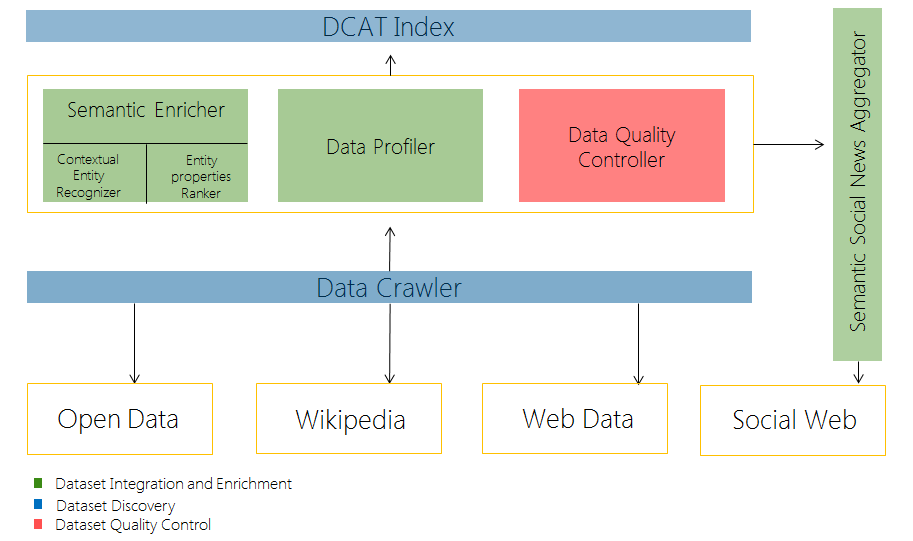
\includegraphics[scale=0.5]{architecture_diagram.png}
  \caption{Overall Architecture}
  \label{fig:architecture_diagram}
\end{figure}

 \begin{itemize}
 \item {\bf Data Acquisition}: Be able to sample data from the various structured data sources like Wikipedia tables, Open data portals, etc. While these are rich sources of information, sometimes live information streamed from the Social Networks is needed. As a result, we crawl Social Networks in order to aggregate semantically related information and connect it with the right resources.
 \item {\bf Data Preparation}: This includes data profiling and validation, de-duplicating and enhancing relevant data sets with metadata. Profiling is used to examine data to understand its content, structure and data quality dependencies. The types of profiling tasks include:
 \begin{itemize}
 \item Examining column data and getting statistical information such as min, max, average, median, null percentage, value distribution, pattern distribution.
 \item Dependency tasks: Finds the values in one or more dependent columns that rely on values in a primary column
 \item Redundancy tasks: Determine the degree of overlapping data values or duplication between two sets of columns
 \item Uniqueness tasks: Returns the count and percentage of rows that contain non-unique data, for the set of column(s) selected.
 \item Content type: Content type profiling provides suggested meaning based on the entities data in the columns.
 \item Quality checks: An important aspect that we have to take into consideration while describing a dataset is its quality. For that, an objective Linked Data quality assessment framework should be created in order to issue quality profiles that extend the DCAT vocabulary. The framework helps on one hand data owners to rate the quality of their dataset and get some hints on possible improvements, and on the other hand data consumers to choose their data sources from a ranked set.
 \end{itemize}
 \item {\bf Dataset Classification}: Classify and organize datasets based on the input from the previous tasks.
\end{itemize}

\subsection{Contributions on Dataset Integration and Enrichment}
Regarding this aspect of our research, we have achieved the following tasks:
 \begin{itemize}
 \item Building RUBIX which is a framework enabling mash-up of potentially noisy enterprise and external data.
 \item RUBIX improves instance and schema matching by adding Semantic metadata to data at the instance level.
 \item RUBIX improves data integration techniques by enabling clean representation of the data regardless of the languages used, existence of abbreviations, synonyms and typos.
 \item Build a Social crawler that queries several Social endpoints and aggregates news based on a set of defined keywords.
 \item Build a common Semantic model to represent Web documents.
 \item Building a Semantic Social News Aggregating service (SNARC)~\cite{Assaf:ESWC:13} that aggregates relevant Social news with regards to a Web document.
 \item Reverse engineering of Google Knowledge Graph Panel in order to define the top properties of a selected entity.
 \item High traction from the BI organization to integrate it as a service into various offerings.
 \item We presented RUBIX at the First International Workshop on Open Data~\cite{Assaf:WOD:12}.
 \item SNARC has won the first place at the AI Mashup Challenge\footnote{\url{http://aimashup.org/aimashup13}} at ESWC13.
\end{itemize}

\subsection{Contributions on Dataset Quality Control}
Concerning our contributions on Linked Data quality assessment, we have achieved the following tasks:
\begin{itemize}
\item We identified five principle classes to describe the quality of a particular linked dataset. For each class, we list the principles that are involved at all stages of the data management process.
\item We have presented our Data quality principles at the Sixth IEEE International Conference on Semantic Computing~\cite{Assaf:DQMST:12}.
\item We have surveyed the landscape of Linked Data quality assessment frameworks.
\item We have surveyed the landscape of Linked Data quality assessment tools.
\item We have refined the five principles in~\cite{Assaf:DQMST:12} towards a more objective framework.
\item We have evaluated the surveyed tools with regards to the suggested framework.
\end{itemize}

%%%%%%%%%%%%%%%%%%%%%%%%%%%%%%%%%%%%
%%% Dataset Integration and Enrichment %%%
%%%%%%%%%%%%%%%%%%%%%%%%%%%%%%%%%%%%

\section{Dataset Integration and Enrichment}
\label{sec:dataset_integration_and_enrichment}

Tagging and attaching metadata is often seen as additional work for data publishers with few paybacks. Moreover, different data creators use different terminologies which means that the same object maybe be represented using different metadata descriptions~\cite{Furnas:ACM:87}. Presenting and enterprise taxonomies requires a considerable amount of time and effort, at least in the initial creation steps~\cite{Frischmuth:SemWebJorunal:12}.

\subsection{What are the Important Properties of an Entity}
In many knowledge bases, entities are described with numerous properties. However, not all properties have the same importance. Some properties are considered as keys for performing instance matching tasks while other properties are generally chosen for quickly providing a summary of the key facts attached to an entity. Our motivation is to provide a method enabling to select what properties should be used when depicting the summary of an entity, for example when augmenting extra columns into an existing dataset or when annotating instances with semantic tags.

Our approach consists in: (i) reverse engineering the Google Knowledge Panel by extracting the properties that Google considers as sufficiently important to show and (ii) analyzing users' preferences by conducting a user survey and comparing the results.

We have shown that it is possible to reveal what are the ``important'' properties of entities in a large knowledge base by reverse engineering the choices made by Google when creating knowledge graph panels and by comparing with users preferences obtained from a user survey. Our motivation is to represent this choice explicitly, using the Fresnel vocabulary, so that any application could just read this configuration file for deciding which properties of an entity is worth to visualize. We are aware that this knowledge is highly dynamic, the Google Knowledge Graph panel differing from countries and varying along the time. We have provided the code that enables to perform new calculation at run time and we aim to study the temporal evolution of what are important properties on a longer period. This knowledge which has been captured will be made available shortly in a SPARQL endpoint. We are also investigating the use of Mechanical Turk to perform a larger survey for the complete set of DBpedia classes.

\subsection{Semantic Enrichment of Data}

RUBIX is our approach to bootstrap the process of attaching meta information to data objects. We leverage DBpedia and Freebase as knowledge bases for our annotation process. In RUBIX we assign a vector of Semantic types for every object at the instance level. For example, Orange will be represented by a vector of rich types that contain \texttt{(Organization, Organism Classification, Place ...)}. Currently, we rely on Freebase API to identify these rich types, but we have already started the effort to build an entity type ranking tool inspired by~\cite{Tonon:ISWC:13}.

\subsection{RUBIX to Enhance Schema Matching}

In the past, some work has tried to improve existing data schema~\cite{Miller:IEEE:03} but literature mainly covers automatic or semi-automatic labeling of anonymous data sets through Web extraction. Examples include~\cite{Reis:WWW:04} that automatically labels news articles with a tree structure analysis or~\cite{Wang:WWW:03} that defines heuristics based on distance and alignment of a data value and its label. These approaches are however restricting label candidates to Web content from which the data was extracted.~\cite{DaSilva:OTM:07} goes a step further by launching speculative queries to standard Web search engines to enlarge the set of potential candidate labels. More recently,~\cite{Limaye:VLDB:10} applies machine learning techniques to respectively annotate table rows as entities, columns as their types and pairs of columns as relationships, referring to the YAGO ontology. The work presented aims however at leveraging such annotations to assist semantic search queries construction and not at improving schema matching.
With the emergence of the Semantic Web, new work in the area has tried to exploit Linked Data repositories. The authors of~\cite{Syed:WebSci:10} present techniques to automatically infer a semantic model on tabular data by getting top candidates from Wikitology~\cite{Finin:AAAI:09} and classifying them with the Google page ranking algorithm. Since the authors' goal is to export the resulting table data as Linked Data and not to improve schema matching, some columns can be labeled incorrectly, and acronyms and languages are not well handled~\cite{Syed:WebSci:10}. In the Helix project~\cite{Hassanzadeh:WWW:11}, a tagging mechanism is used to add semantic information on tabular data. A sample of instances values for each column is taken and a set of tags with scores are gathered from online sources such as Freebase. Tags are then correlated to infer annotations for the column. The mechanism is quite similar to ours but the resulting tags for the column are independent of the existing column name and sampling might not always provide a representative population of the instance values.

In RUBIX we have implemented several matching algorithms (Cosine Similarity, Pearson Product-Moment Correlation Coefficient (PPMCC) and Spearman's Rank Correlation Coefficient) in order to calculate similarity between data based on their rich types population. Our preliminary evaluation shows that for datasets where mappings were relevant yet not proposed, our framework provides higher quality matching results. Additionally, the number of matches discovered is increased when Linked Data is used in most datasets.

\subsection{Dataset Annotation and Domain Identification}

The increasing diversity of the datasets makes it difficult to annotate them with a fixed number of pre-defined tags. Moreover, manually entered tags are subjective and may not capture the essence and breadth of the dataset~\cite{Lalithsena:WI:13}. RUBIX can be used to Annotate datasets with meta information based on examining the data instances themselves. In addition to that, we can enhance our approach by applying techniques similar to~\cite{Lalithsena:WI:13} in order to identify topical domains with fine-grained classification.

%%%%%%%%%%%%%%%%%%%%%%%%%%%%%%%%%%%%
%%%  Semantic Social News Aggregation %%%
%%%%%%%%%%%%%%%%%%%%%%%%%%%%%%%%%%%%
\subsection{Semantic Social News Aggregation (SNARC)}

The Internet has created a paradigm shift in how we consume and disseminate information. Data nowadays is spread over heterogeneous silos of archived and live data. People willingly share data on social media by posting news, views, presentations, pictures and videos. SNARC is a service that uses semantic web technology and combines services available on the web to aggregate social news. SNARC brings live and archived information to the user that is directly related to his active page. The key advantage is an instantaneous access to complementary information without the need to dig for it. Information appears when it is relevant enabling the user to focus on what is really important.

Crawling data from these heterogeneous platforms implies the studying of related API specifications which differ in terms of use, privacy policy and described methods. Harvesting content spread over multiple platforms is a challenging task that has to ensure an easy and flexible way for integrating several social Web APIs. Tools such as API Blender~\cite{Gouriten:WWW:12} or Media Finder~\cite{Hyunmo:HCI:03} provide such interface with the aim to save developers' efforts for learning each API specification. However, for in SNARC we needed services that are not available in the mentioned services. As a result, we have implemented our own Social crawler for Twitter\footnote{\url{http://www.twitter.com}}, Google+\footnote{\url{http://plus.google.com}}, YouTube\footnote{\url{http://www.youtube.com}}, Vimeo\footnote{\url{http://www.vimeo.com}}, Slideshare\footnote{\url{http://www.slideshare.com}}, Stack Exchange \footnote{\url{http://stackexchange.com/}}and the Web.


%%%%%%%%%%%%%%%%%%%%%%%%%%%%%%%%%%%%
%%% Dataset Quality Control %%%
%%%%%%%%%%%%%%%%%%%%%%%%%%%%%%%%%%%%

\section{Dataset Quality Control}
\label{sec:dataset_quality_control}
We are entering an era where open is the new default. Governments, universities, organizations and even individuals are publicly publishing huge amounts of open data.  This openness should be accompanied with a certain level of trust or guarantees about the quality of data.  To our knowledge, only one certificate is available to data publishers to assess the quality level of their datasets, the ODI certificate\footnote{\url{https://certificates.theodi.org/}}.

This certificate provides a description of the published data quality in plain English. It aspires to act as a mark of approval that helps publishers understand how to publish good open data and users how to use it. It gives publishers the ability to provide assurance and support on their data while encouraging further improvements through an ascending scale.

ODI comes as an online and free questionnaire for data publishers focusing on certain characteristics about their data. The questions are classified into the following categories: general information (about dataset, publisher and type of release), legal information (e.g., rights to publish), licensing, privacy (e.g., whether individuals can be identified), practical information (e.g., how to reach the data), quality, reliability, technical information (e.g., format and type of data) and social information (e.g., contacts, communities, etc.). Based on the information provided  by the data  publisher,  a certificate  is created  with one of four different ratings.

Although ODI is a great initiative, the issued certificates are “self-certified“. ODI does not verify or review submissions but retains the right to revoke a certificate at any time. The dynamicity of Linked Data  makes it also very difficult to update the certificates manually, especially when these changes are frequent and affect multiple categories. There is clearly a need for automatic certification which can be supplemented with some manual input for categories that cannot be processed by machines.


The emerging critical need for large, distributed, heterogeneous, and complex structured datasets identified the necessity to establish industry cooperation between vendors of RDF and Graph database technologies in developing, endorsing, and publishing reliable and insightful benchmark results. The Linked Data Benchmark Council (LDBC)\footnote{\url{http://ldbc.eu/}} aims to bridge the gap between the industry and the new trending stack of semantic technologies and their vendors.

LDBC more specifically aims at developing new benchmarks that will lead to significant progress in scalability, storage, indexing and query optimization techniques to become the de facto standard for publishing performance results. LDBC is promising initiative, but it is still work in progress with the final report expected on the first quarter of 2015.

In addition to the initiatives mentioned above, there exists a number of data quality frameworks and tools that are either standalone or implemented as modules in data integration tools.

LODGRefine\footnote{\url{http://code.zemanta.com/sparkica/}} is the Open Refine\footnote{\url{http://openrefine.org/}} of Linked Data. It does not act as a quality assessment tool, but it is powerful in cleaning and refining raw instance data. LODGRefine can help detect duplicates, empty values, spot inconsistencies, extract Named Entities, discover patterns and more. LODGRefine helps in improving the quality of the dataset by improving the quality of the data at the instance level.


PROLOD~\cite{Bohm:ICDEW:10} is also not a quality assessment tool. It is a Linked Data profiling tool that provides clustering and labeling capabilities, schema discovery and statistics about data types and patterns. The statistics are about properties distribution, link-to-literal ratio, number of entities and RDF triples, average properties per entity and average error. PROLOD had been tested with DBpedia but the authors plan to improve its scalability to larger datasets.


Sieve~\cite{Mendes:EDBT:12} is framework for expressing quality assessment and fusion methods. It is implemented as a component of the Linked Data Integration Framework (LDIF)\footnote{\url{http://ldif.wbsg.de/}}. Sieve leverages the LDIF provenance metadata as quality indicators to produce quality assessment scores. However, despite its nice features, it is only targeted to perform data fusion based on user-configurable conflict resolution tasks. Moreover, since Sieve main input is provenance metadata, it is only limited to domains that can provide such metadata associated with their data.


Quality Assessment of Data Sources (Flemming's Data Quality Assessment Tool)\footnote{\url{http://linkeddata.informatik.hu-berlin.de/LDSrcAss/datenquelle.php}} calculates data quality scores based on manual user input. The user should assign weights to the predefined quality metrics and answer a series of questions regarding the dataset. These include, for example, the use of obsolete classes and properties by defining the number of described entities that are assigned disjoint classes, the usage of stable URIs and whether the publisher provides a mailing list for the dataset. The main disadvantage for using this tool is the manual intervention which requires deep knowledge in the dataset examined. Moreover, the tool lacks support for several quality concerns like completeness or consistency.


SWIQA~\cite{Furber:ECIS:11} is composed of three layers: data acquisition, query and ontology layers. It uses query templates based on the SPARQL Inferencing Notation (SPIN)\footnote{\url{http://spinrdf.org/}} to express quality requirements. The queries are built to compute weighted and unweighted quality scores. At the end of the assessment, it uses vocabulary elements to annotate important values of properties and classes, assigning inferred quality scores to ontology elements and classifying the identified data quality problems.

Despite all the recent efforts in providing frameworks and tools for data quality in Linked Open Data, there is still no framework for the objective assessment of such quality taking into account all aspects of Linked Open Data.

In our previous work~\cite{Assaf:DQMST:12} we have identified 24 different Linked Data quality attributes. We have refined these attributes into a condensed framework of 13 objective attributes. Since these attributes are rather abstract, we should rely on quality indicators that reflect data quality~\cite{Flemming:Thesis:10}. In this paper, we transform the quality indicators presented as a set of questions in~\cite{Assaf:DQMST:12} into more concrete quality indicator metrics. We extend them with the the objective quality indicators listed in the systematic review done in~\cite{Zaveri:SemWebJorunal:12}.

As a result, we have identified the need for a complete quality framework that can assess all the quality indicators. Most of the tools were designed with limited coverage to certain aspects, for example, ontology and vocabulary checkers focus mainly on the coherence, completeness and correctness at the modeling level. Flemming's tool covers several attributes like the completeness, correctness, conciseness, security, licensing and comprehensibility, but it falls short in measuring the consistency, coherence, efficiency and provenance.

We have also noticed the lack of tools to measure certain quality indicators like the dataset's security. Moreover, to our knowledge, there are no tools that can measure all the provenance quality indicators (except for Flemming's tool that is able to check for the use of digital signatures) although the literature covers several approaches to achieve that~\cite{Hartig:ISWC:09}\cite{Flouris:EvoDyn:12}\cite{Harth:ISWC:09}.

%%%%%%%%%%%%%%%%%%%%%%%%%%%%%%%%%%%%
%%%  Conclusions and Future Work %%%
%%%%%%%%%%%%%%%%%%%%%%%%%%%%%%%%%%%%

\section{Conclusions and Future work}
\label{sec:conclusion_and_future_work}

We have presented in this document our main contributions in some issues around Enriching Enterprise Data Towards self-service Data Provisioning. We have first focused on the aspect of data profiling through RUBIX. We plan to extend RUBIX to be able to work with DBpedia leveraging the planned entity type ranking module. We also plan to include data mining techniques to profile numerical data and provide statistical insights about data distribution.

Regarding the Linked Data quality module, we plan to develop a comprehensive objective Linked Data quality evaluation tool. The tool will be able to automatically measure the various quality indicators listed in this paper, introduce a scoring function with different weights for the various quality attributes and issue a quality certificate.

Regarding the Social integration, we would like to test SNARC on business web application, check if our annotations can be used to successfully query and attach relevant social snippets to the data.

We also plan to build our Linked Data crawler that will be responsible for the data acquisition phase which is the entry point for the work done so far. We also plan to investigate possible extensions to the current data description vocabularies to allow more comprehensive datasets categorization.


\bibliographystyle{amsplain}
\bibliography{../../Util/Bibliography/bibliography}

\end{document}
